\documentclass{beamer}
\usepackage{beamerthemesplit}
\usepackage{booktabs}
\usepackage{graphicx}
\usepackage{transparent}
\usepackage[italian]{babel}
\usepackage[utf8x]{inputenc}
\usepackage{listings}
\usepackage{tikz}
\usepackage{amsfonts}
\usetikzlibrary{arrows,shapes}
\tikzstyle{actor edge} = [red!90]
\tikzstyle{director edge} = [blue!90]
\usepackage{pgfplots}
\usepackage{scalefnt}
\definecolor{gold}{RGB}{255, 215, 0}
\definecolor{silver}{RGB}{192,192,192}
\definecolor{bronze}{RGB}{205, 127, 50}
\usepackage{color}
\usepackage{xcolor}
\definecolor{var}{RGB}{20,105,176}
\colorlet{prefix}{magenta!60!black}
\colorlet{keyword}{red!60!black}
\lstdefinelanguage{customized}{
	basicstyle=\fontsize{8}{10}\selectfont \ttfamily,%
	columns=fullflexible,%
	showstringspaces=false,%
	breaklines=true,%
	frame=lines,%
	xleftmargin=10mm, %
	xrightmargin=25mm, %
	breakatwhitespace=false, %
	tabsize=2, %
	captionpos=b, %
 literate=
 *{PREFIX}{{{\color{keyword}{PREFIX }}}}{1}
 {SELECT}{{{\color{keyword}{SELECT }}}}{1}
 {FROM}{{{\color{keyword}{FROM }}}}{1}
 {WHERE}{{{\color{keyword}{WHERE }}}}{1}
 {?name}{{{\color{var}{?name}}}}{1}
 {dbpedia: }{{{\color{prefix}{dbpedia:}}}}{1}
 {prop: }{{{\color{prefix}{prop:}}}}{1}
}

\title[LOD CB-RS]{Linked Open Data per un Content-based Recommender System}
\institute{ \textbf{Accesso intelligente alle informazioni ed \\ elaborazione del linguaggio naturale\\}
~ \\
\begin{small}
Corso di Laurea in Informatica Magistrale
\end{small}}
\author{\textbf{Luciano Quercia}\\
\textbf{Simone Rutigliano}}
\date{\tiny{\today}}

\usebackgroundtemplate{
%    \transparent{0.12}{
     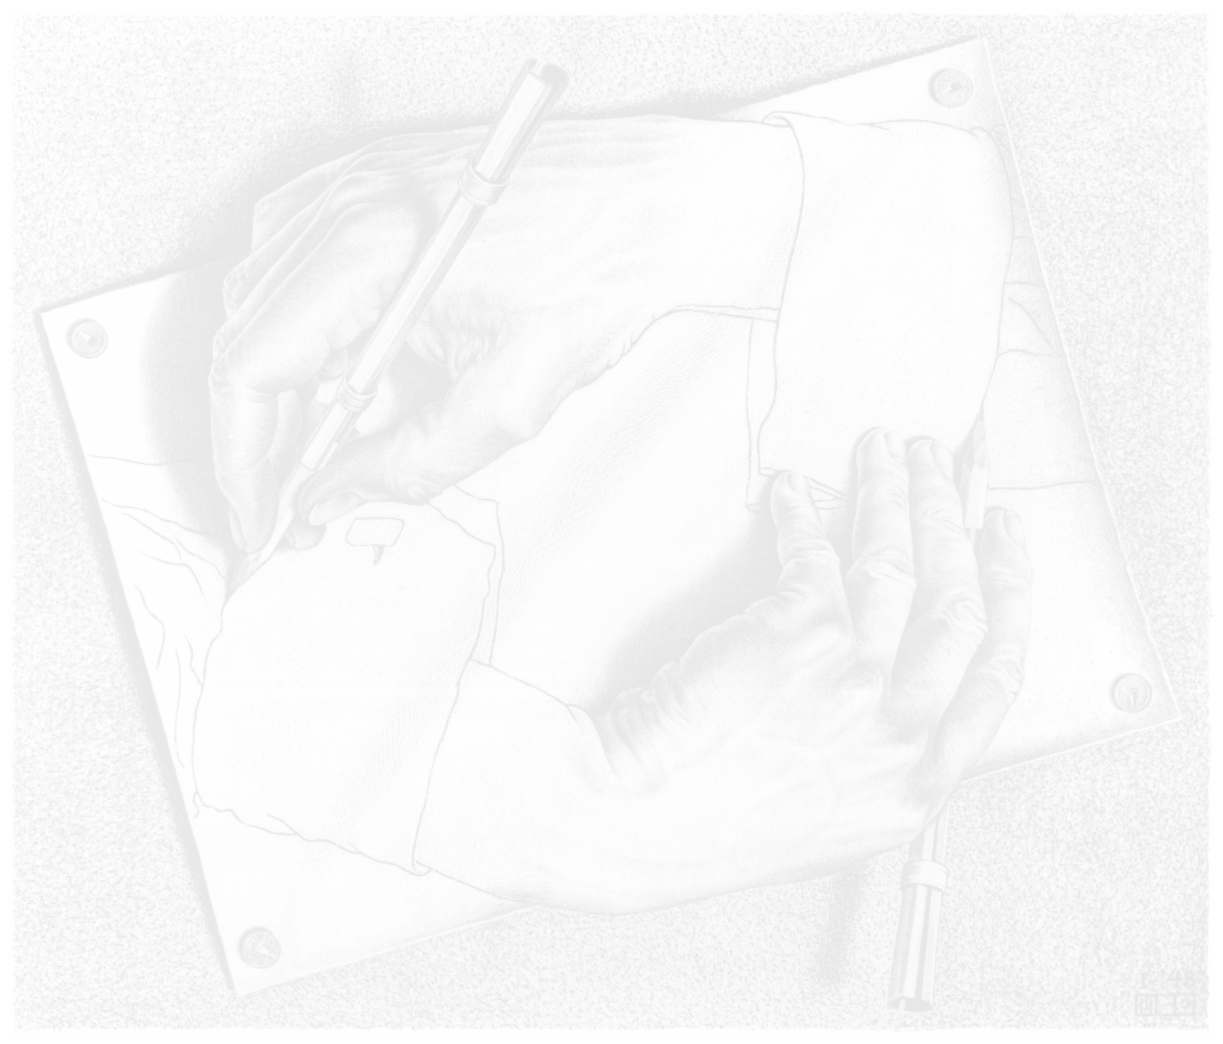
\includegraphics[width=\paperwidth, height=\paperheight]{./figure/escher_hands_tr.png}
%    }
}

%\usetheme{Hannover}
\usetheme{Copenhagen}
\usecolortheme{seahorse}
\usecolortheme{rose}
%\usetheme{Frankfurt}
%\usecolortheme{beetle}

%\useoutertheme[subsection=false]{smoothbars}
%\useoutertheme[subsection=false]{smoothtree}
\useoutertheme{shadow}
\setbeamercovered{dynamic}

\pgfdeclareimage[height=1cm]{logo}{figure/logo}
\logo{\pgfuseimage{logo}}

\usetikzlibrary{arrows,shapes}
\tikzstyle{vertex}=[circle,fill=black!25,minimum size=20pt,inner sep=0pt]
\tikzstyle{selected vertex} = [vertex, fill=red!24]
\tikzstyle{edge} = [draw,thick,-]
\tikzstyle{weight} = [font=\small]
\tikzstyle{selected edge} = [draw,line width=5pt,-,red!50]
\tikzstyle{ignored edge} = [draw,line width=5pt,-,black!20]


\begin{document}

%%%%%%%%%%%%%%%%%%%%%%%%%%%%%%%%%%%%%%%%%%%%%%%%%%%%%

\begin{frame}
\maketitle
\end{frame}

%%%%%%%%%%%%%%%%%%%%%%%%%%%%%%%%%%%%%%%%%%%%%%%%%%%%%

\begin{frame}
\frametitle{Outline}
	\tableofcontents
\end{frame}

%%%%%%%%%%%%%%%%%%%%%%%%%%%%%%%%%%%%%%%%%%%%%%%%%%%%%

\section{Obiettivi}
\begin{frame}
\frametitle{Obiettivi}
Realizzazione di un \textbf{content-based recommender system}

basato sulla \textbf{Linked Open Data Cloud}
\end{frame}

%%%%%%%%%%%%%%%%%%%%%%%%%%%%%%%%%%%%%%%%%%%%%%%%%%%%%

\begin{frame}
\frametitle{Content-based Recommender System}
Il sistema stabilisce a priori la distanza trai film al fine di raccomandare i più simili alle preferenze dell'utente

\begin{figure}
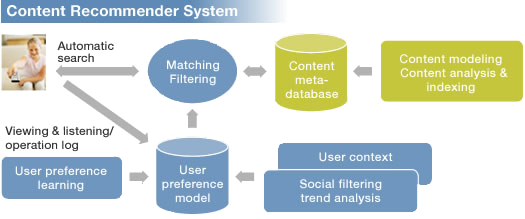
\includegraphics[width=.8\textwidth]{figure/cbrs.png}
\end{figure}

\end{frame}

%%%%%%%%%%%%%%%%%%%%%%%%%%%%%%%%%%%%%%%%%%%%%%%%%%%%%

\begin{frame}
\frametitle{Linked Open Data Cloud}

%
\includegraphics[width=.95\textwidth]{figure/LoDLogo.png}

Collezione (\textbf{Cloud}) di dataset:
\begin{itemize}
\item descritti attraverso RDF
\item fortemente interconnessi fra loro (\textbf{Linked})
\item fruibili liberamente e gratuitamente (\textbf{Open})
\end{itemize}
\end{frame}

%%%%%%%%%%%%%%%%%%%%%%%%%%%%%%%%%%%%%%%%%%%%%%%%%%%%%

\begin{frame}
\frametitle{Linked Open Data Cloud}
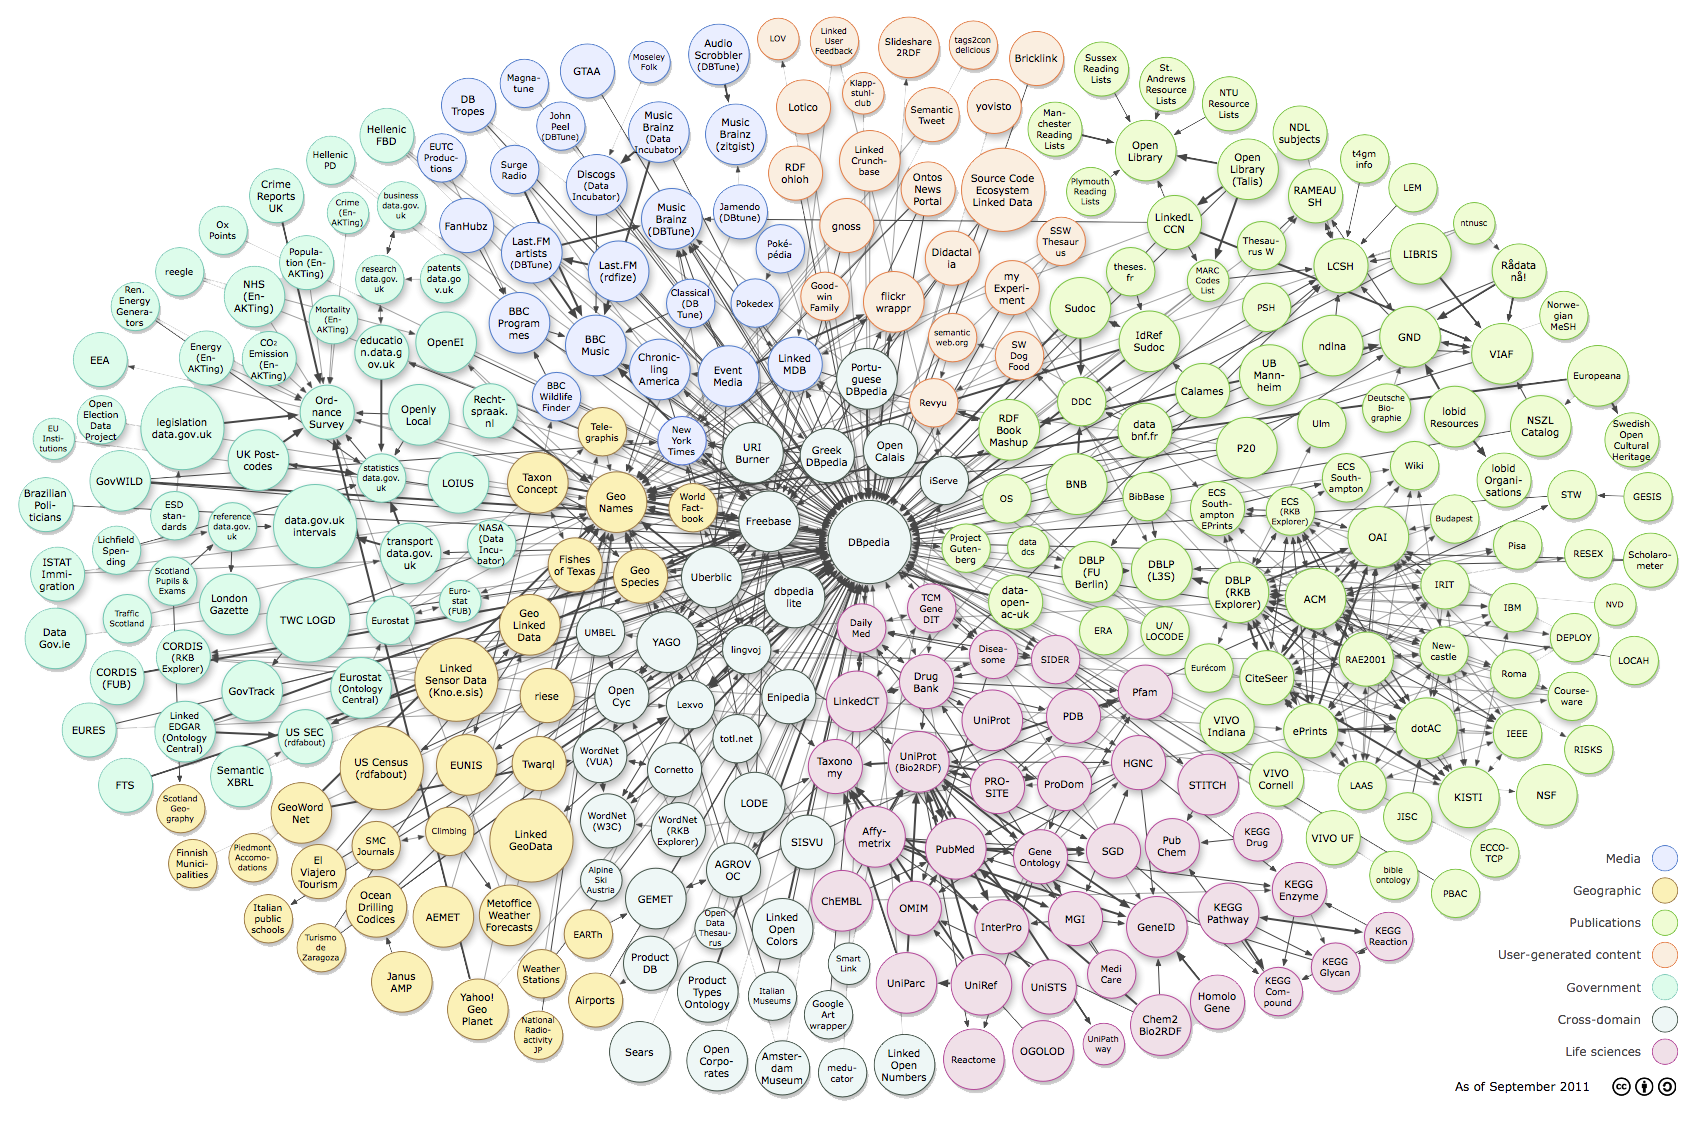
\includegraphics[width=.95\textwidth]{figure/lodcloud}
\end{frame}

%%%%%%%%%%%%%%%%%%%%%%%%%%%%%%%%%%%%%%%%%%%%%%%%%%%%%

\begin{frame}
\frametitle{Resource Description Framework}
Strumento base proposto da \emph{W3C} per la codifica, lo scambio e il riutilizzo di metadati strutturati.

L'RDF Data Model si basa su tre principi chiave:
\begin{enumerate}
\item qualunque cosa può essere identificata da un URI
\item utilizzare il linguaggio meno espressivo per definire qualunque cosa
\item qualunque cosa può dire qualunque cosa su qualunque cosa
\end{enumerate}
\end{frame}

%%%%%%%%%%%%%%%%%%%%%%%%%%%%%%%%%%%%%%%%%%%%%%%%%%%%%

\begin{frame}
\frametitle{Esempio - Resource Description Framework}
Considerando la frase:\\~\\
\begin{center} \emph{Tarantino is the director of the Django Unchained.} \\~\\
\end{center}
L'affermazione può essere suddivisa come: \\~\\
\begin{tabular}{ l | l }
 Soggetto (Risorsa) & Django Unchained \\
 Predicato (Proprietà) & director \\
 Oggetto (Risorsa) & Tarantino \\
\end{tabular}
\end{frame}

%%%%%%%%%%%%%%%%%%%%%%%%%%%%%%%%%%%%%%%%%%%%%%%%%%%%%

\section{Progetto}

\subsection{Sorgente dati}

\begin{frame}
\frametitle{DBPedia}
\begin{columns}

\begin{column}{0.4\textwidth}
\vspace{1cm}
\centering
\includegraphics[width=.8\textwidth]{figure/dbpedialogo}
\begin{itemize}
\item Centro della Linked Open Data Cloud
\item Dump di Wikipedia trasformato in RDF
\end{itemize}
\end{column}
\begin{column}{0.6\textwidth}
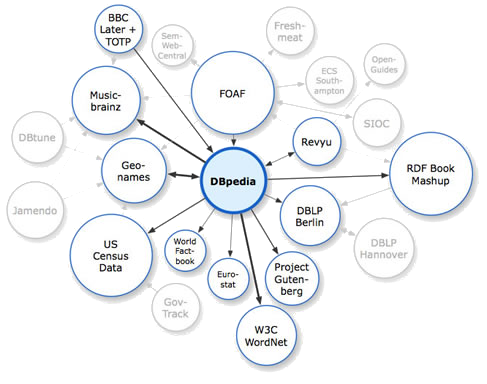
\includegraphics[width=1\textwidth]{figure/AboutDBPedia}
\end{column}
\end{columns}
\end{frame}

%%%%%%%%%%%%%%%%%%%%%%%%%%%%%%%%%%%%%%%%%%%%%%%%%%%%%

\begin{frame}
\frametitle{Proprietà estratte}
Per la raccomandazione di film, abbiamo estratto le seguenti proprietà
\begin{columns}
\begin{column}{0.5\textwidth}
\begin{itemize}
\item studio
\item music
\item music composer
\item writer
\item editing
\item director
\end{itemize}
\end{column}
\begin{column}{0.5\textwidth}
\begin{itemize}
\item subject
\item starring
\item productor
\item writer
\item cinematography
\end{itemize}
\end{column}
\end{columns}
\end{frame}

%%%%%%%%%%%%%%%%%%%%%%%%%%%%%%%%%%%%%%%%%%%%%%%%%%%%%

\subsection{Realizzazione}

%%%%%%%%%%%%%%%%%%%%%%%%%%%%%%%%%%%%%%%%%%%%%%%%%%%%%

\begin{frame}[fragile]
\frametitle{Grafo delle Risorse}
Attraverso query SPARQL\footnote{\emph{Endpoint} : \url{http://dbpedia.org/sparql}} sono state estratte tutte le triple RDF aventi come predicato una delle proprietà definite in precedenza. \\~\\
\begin{lstlisting}[language=customized]
PREFIX dbpedia: http://dbpedia.org/resource/
PREFIX prop: http://dbpedia.org/ontology/
SELECT ?name
WHERE {
 dbpedia:Django_Unchained prop:director ?name .
}
\end{lstlisting}
risultato:

\begin{lstlisting}[language=customized]
http://dbpedia.org/resource/Quentin_Tarantino
\end{lstlisting}
\end{frame}

%%%%%%%%%%%%%%%%%%%%%%%%%%%%%%%%%%%%%%%%%%%%%%%%%%%%%

\begin{frame}
\frametitle{Grafo delle Risorse} 
Esempio di grafo delle risorse ottenuto partendo dalle triple RDF estratte precedentemente. \\~\\
\begin{columns}[p]
\begin{column}{0.8\textwidth}
\begin{tikzpicture}
[lineDecorate/.style={-,thick},%
actor/.style={shape=circle,inner sep=3pt,draw, thick},
film/.style={shape=diamond,inner sep=4pt,draw,thick, fill=blue!15}]

%% nodes or vertices
\foreach \nodename/\x/\y/\direction/\navigate in {
$Django Unchained$/1/3/left/west, $Inglourious Basterds$/3/3/right/east, $Titanic$/1/1/left/west, $Avatar$/3/1/right/east}
{
\node (\nodename) at (\x,\y) [film] {};
\node [\direction] at (\nodename.\navigate) {\footnotesize$\nodename$};
}

\foreach \nodename/\x/\y/\direction/\navigate in {
$Quentin Tarantino$/2/4/above/north, $Leonardo Di caprio$/1/2/left/west, $Christoph Waltz$/3/2/right/east, $James Cameron$/2/0/below/south}
{
\node (\nodename) at (\x,\y) [actor] {};
\node [\direction] at (\nodename.\navigate) {\footnotesize$\nodename$};
}

%% edges or lines
\path
\foreach \startnode/\endnode in {$Django Unchained$/$Leonardo Di caprio$, $Django Unchained$/$Christoph Waltz$, $Inglourious Basterds$/$Christoph Waltz$, $Leonardo Di caprio$/$Titanic$}
{
(\startnode) edge[lineDecorate,actor edge] node {} (\endnode)
}

\foreach \startnode/\endnode in {$Django Unchained$/$Quentin Tarantino$,$Quentin Tarantino$/$Inglourious Basterds$}
{
(\startnode) edge[lineDecorate,bend left,director edge] node {} (\endnode)
}

\foreach \startnode/\endnode in {$Quentin Tarantino$/$Django Unchained$, $Inglourious Basterds$/$Quentin Tarantino$}
{
(\startnode) edge[lineDecorate,bend left,actor edge] node {} (\endnode)
}

\foreach \startnode/\endnode in {$Avatar$/$James Cameron$,$James Cameron$/$Titanic$}
{
	(\startnode) edge[lineDecorate,bend left,director edge] node {} (\endnode)
};

\end{tikzpicture}
\end{column}

\begin{column}{0.35\textwidth}
\begin{tabular}{l l}
\begin{tikzpicture}[film/.style={shape=diamond,inner sep=3pt,draw,thick, fill=blue!15}]
 \node (a) at (6,3) [film] {};
 \node [right] at (a.west) {\footnotesize};
\end{tikzpicture}
& Film \\

\begin{tikzpicture}[actor/.style={shape=circle,inner sep=3pt,draw, thick}]
 \node (a) at (9,3) [actor] {};
 \node [right] at (a.west) {\footnotesize};
\end{tikzpicture}
& Resource \\

\color{blue}--- & Edge director \\
\color{red}--- & Edge actor \\
\end{tabular}

\end{column}
\end{columns}
\end{frame}

%%%%%%%%%%%%%%%%%%%%%%%%%%%%%%%%%%%%%%%%%%%%%%%%%%%%%

\begin{frame}
\frametitle{Grafo dei Film}
Tutte le risorse non film sono state epurate ed inglobate all'interno degli archi.
\\~\\
\begin{tikzpicture}
[lineDecoratein/.style={<-,thick}, %
lineDecorateout/.style={->,thick}, %
lineDecorate/.style={<->,thick},%
film/.style={shape=diamond,inner sep=4pt,draw,thick, fill=blue!15}]

%% nodes or vertices
\foreach \nodename/\x/\y/\direction/\navigate in {
$Django Unchained$/0/4/left/west, $Inglourious Basterds$/4/4/right/east, $Titanic$/0/1/left/west, $Avatar$/4/1/right/east}
{
\node (\nodename) at (\x,\y) [film] {};
\node [\direction] at (\nodename.\navigate) {\small$\nodename$};
}
\node ($actor Di Caprio actor$) at (0,2) {\color{red}\scriptsize{actor Di Caprio actor}};

%% edges or lines
\path
\foreach \startnode/\endnode in {$Django Unchained$/$actor Di Caprio actor$}
{
(\startnode) edge[lineDecoratein,actor edge] node[] {} (\endnode)
}

\foreach \startnode/\endnode in {$Titanic$/$Avatar$}
{
	(\startnode) edge[lineDecorate,director edge] node[auto] {\scriptsize{director Cameron director}} (\endnode)
}

\foreach \startnode/\endnode in {$actor Di Caprio actor$/$Titanic$}
{
	(\startnode) edge[lineDecorateout,actor edge] node[] {} (\endnode)
}

\foreach \startnode/\endnode in {$Django Unchained$/$Inglourious Basterds$}
{
(\startnode) edge[lineDecorate,bend left,actor edge] node[auto] {\scriptsize{actor Tarantino actor}} (\endnode)
}

\foreach \startnode/\endnode in {$Inglourious Basterds$/$Django Unchained$}
{
(\startnode) edge[lineDecorate,bend left,director edge] node[auto] {\scriptsize{director Tarantino director}} (\endnode)
};

\end{tikzpicture}
\end{frame}

%%%%%%%%%%%%%%%%%%%%%%%%%%%%%%%%%%%%%%%%%%%%%%%%%%%%%

\subsection{Fattori}

%%%%%%%%%%%%%%%%%%%%%%%%%%%%%%%%%%%%%%%%%%%%%%%%%%%%%

\begin{frame}
\frametitle{Distanze}
Sono state applicate 4 tipi di distanze di Passant sul grafo:

\begin{columns}

\begin{column}{.25\paperwidth}
\begin{itemize}
\item<1> Direct
\vspace{.6cm}
\item<2> Combinated
\vspace{.6cm}
\item<3> Direct Weighted
\vspace{.6cm}
\item<4> Combinated Weighted
\end{itemize}
\end{column}

\begin{column}{.65\paperwidth}

\only<1>{\begin{block}{Direct}\footnotesize{
$$P_{d}(f_{a},f_{b}) = \frac{1} {1+C_{d}(f_{a},f_{b})+C_{d}(f_{b},f_{a})}$$

$$C_{d}(f_a,f_b) = \left\vert \left\{ e \in Edges \  | \  (f_a \xrightarrow{~e~} f_b ) \right\} \right\vert$$
}\end{block}}

\only<2>{\begin{block}{Combinated}\tiny{
$$P_{c}(f_{a},f_{b}) = \frac{1} {1+C_{d}(f_{a},f_{b})+C_{d}(f_{b},f_{a})+C_{io}(f_{a},f_{b})+C_{ii}(f_{a},f_{b})}$$
\vspace{.4cm}
$$C_{io}(f_a,f_b) = \left\vert \left\{ f \  | \  (f_a \xrightarrow{~e~} f ) \wedge (f_b \xrightarrow{~e~} f) \right\} \right\vert$$
$$C_{ii}(f_a,f_b) = \left\vert \left\{ f \  | \  ( f \xrightarrow{~e~} f_a ) \wedge ( f \xrightarrow{~e~} f_b) \right\} \right\vert$$
$$\text{con} \ e \in Edges  , \qquad f_a,f_b,f \in Films$$
}\end{block}}

\only<3>{\begin{block}{Direct Weighted}\scriptsize{
$$
P_{dw}(f_a,f_b) = \frac{1}{1+CW_{d}(f_a,f_b)+CW_{d}(f_b,f_a)}
$$
$$
CW_{d}(f_a,f_b) = \sum_{e \in ED}^{}{weight(e)}
$$
$$
ED_{f_a,f_b} = \left\{ e \in Edges \quad\big\vert\quad f_a \xrightarrow{~e~} f_b \right\}
$$
}\end{block}}


\only<4>{\begin{block}{Combinated Weighted}\tiny{
$$
P_{cw}(f_{a},f_{b}) = \frac{1} {1+CW_{d}(f_a,f_b)+CW_{d}(f_b,f_a)+CW_{io}(f_a,f_b)+CW_{ii}(f_a,f_b)}
$$
$$
E'_{f_a,f_b} = \left\{ (e_1, e_2) \in Edges \big\vert (f_a \xrightarrow{e_1} f_c) \wedge (f_b \xrightarrow{e_2} f_c) \wedge label(e_1)=label(e_2) \right\}
$$ $$
E''_{f_a,f_b} = \left\{ (e_1, e_2) \in Edges \big\vert (f_c \xrightarrow{e_1} f_a) \wedge (f_c \xrightarrow{e_2} f_b) \wedge label(e_1)=label(e_2) \right\}
$$ $$
CW_{io}(f_a,f_b) = \sum_{(e_1,e_2) \in E'_{f_a,f_b}}{weight(e_1)*weight(e_2)}
$$ $$
CW_{ii}(f_a,f_b) = \sum_{(e_1,e_2) \in E''_{f_a,f_b}}{weight(e_1)*weight(e_2)}
$$
}\end{block}}
\end{column}
\end{columns}
\end{frame}

%%%%%%%%%%%%%%%%%%%%%%%%%%%%%%%%%%%%%%%%%%%%%%%%%%%%%

\begin{frame}
\frametitle{Rappresentazione del profilo}
Il profilo è stato rappresentato in 2 modi:
\begin{center}
\begin{itemize}
	\item \textsc{Simple} - Insieme di film positivi per l'utente
	\pause
	\item \textsc{Weighted} - Ogni film influisce, positivamente o negativamente, alle raccomandazioni, secondo il voto ricevuto
$$
P_{NORM}(f_a) = Voto(f_a)- Voto_M\footnote{Valor medio delle votazioni pari a 3}
$$
\end{itemize}
\end{center}

\end{frame}

%%%%%%%%%%%%%%%%%%%%%%%%%%%%%%%%%%%%%%%%%%%%%%%%%%%%%

\begin{frame}
	\frametitle{Esempio di profilazione}
	considerati i film con le relative votazioni:
	
\begin{center}	
	\begin{tabular}{l c}
		\multicolumn{1}{c}{\textsc{Film}} & \textsc{Votazione} \\
		\hline
		Titanic & 5 \\
		Django Unchained & 4 \\
		Bastardi senza gloria & 2 \\
		\hline
	\end{tabular}
\end{center}	
\medskip
I profili creati saranno:
\begin{center}
\begin{tabular}{l l}
	\textbf{Simple} &
	\begin{tabular}{l}
		Django Unchained \\		
		Titanic \\
	\end{tabular} \\
	\\
	
	\textbf{Weighted} &
	\begin{tabular}{l r}
		%		Film & rilevanza \\
		Titanic & 2 \\
		Django Unchained & 1 \\
		Bastardi senza gloria & -1\\
	\end{tabular}	\\
\end{tabular}
\end{center}	
\end{frame}

%%%%%%%%%%%%%%%%%%%%%%%%%%%%%%%%%%%%%%%%%%%%%%%%%%%%%
\begin{frame}
	\frametitle{Esempio di raccomandazione}
	Data la configurazione:
	\begin{itemize}
		\item \textbf{Profilo} = Weighted 
		\item \textbf{K} = 3
		\item \textbf{Distanza} = Direct Weighted Passant
	\end{itemize} 
\end{frame}
%%%%%%%%%%%%%%%%%%%%%%%%%%%%%%%%%%%%%%%%%%%%%%%%%%%%%

\section{Sperimentazione}
\subsection{Dataset}
\begin{frame}
\frametitle{MovieLens}
Cosa è \textbf{MovieLens}? \\ \vspace{0.5cm}

\href{http://www.grouplens.org/}{\emph{GroupLens Research}}\footnote{\tiny \emph{Gruppo di ricerca del Department of Computer Science and Engineering at the University of Minnesota in ambito di Recommender system algorithms e Information filtering}.} ha raccolto e reso disponibili dei rating datasets estratti dal sito web di \href{http://movielens.umn.edu}{\emph{MovieLens}}.
Il dataset preso in considerazione è composto da 518 film e 613 utenti. Ciascun utente ha votato più film, con una votazione che va da 1 a 5. 
\begin{figure}
	
\includegraphics[width=.3\textwidth]{figure/gl-logo} ~~~~ 
	
\includegraphics[width=.3\textwidth]{figure/movielens-helping}
\end{figure}
\end{frame}
%%%%%%%%%%%%%%%%%%%%%%%%%%%%%%%%%%%%%%%%%%%%%%%%%%%%%

\subsection{Protocollo Sperimentale}

%%%%%%%%%%%%%%%%%%%%%%%%%%%%%%%%%%%%%%%%%%%%%%%%%%%%%

\begin{frame}
\frametitle{Protocollo Sperimentale}
\begin{enumerate}
	\setlength{\itemsep}{10pt}
	\item<1-> Split del set di ogni utente secondo la proporzione 70/30
	\item<2-> Per ogni utente creare:
	\begin{itemize}
		\setlength{\itemsep}{6pt}
		\item[$\diamond$] I due profili utente (pesato e non pesato) utilizzando il Training set
		\item[$\diamond$] Le liste di raccomandazioni, contenente la totalità dei film, ordinate per importanza, secondo le diverse tipologie di distanza
	\end{itemize}
	\item<3-> $\forall k \in (5,10,20,50,100)$ calcolare le metriche\footnote{\emph{Precisione $P_k$ ed MRR}} in base ad ogni combinazione profilo-distanza-Numero di raccomandazione
\end{enumerate}
\end{frame}

%%%%%%%%%%%%%%%%%%%%%%%%%%%%%%%%%%%%%%%%%%%%%%%%%%%%%

\begin{frame}
	\frametitle{Protocollo Sperimentale}
	Combinazioni possibili:
	\begin{columns}[t]
		\begin{column}{0.5\textwidth}
				\begin{itemize}
					\setlength{\itemsep}{10pt}
					\item<1-> \textbf{Distanze}:
					\begin{itemize}
						\item \emph{Passant D}
						\item \emph{Passant C}
						\item \emph{Passant DW}
						\item \emph{Passant CW}
					\end{itemize}
					\item<2-> \textbf{Profili}:
					\begin{itemize}
						\item \emph{Pesato}
						\item \emph{Non Pesato}
					\end{itemize}
				\end{itemize}
		\end{column}
		\begin{column}{0.5\textwidth}
			\begin{itemize}
				\item<3-> \textbf{Numero di raccomandazioni $k$}:
				\begin{itemize}
					\item \emph{5}
					\item \emph{10}	
					\item \emph{20}
					\item \emph{50}
					\item \emph{100}
				\end{itemize}
			\end{itemize}
		\end{column}
	\end{columns}
	\end{frame}

%%%%%%%%%%%%%%%%%%%%%%%%%%%%%%%%%%%%%%%%%%%%%%%%%%%%%

\subsection{Metriche}
\begin{frame}
	\frametitle{Metriche}
	Le metriche utilizzate per valutare il sistema di raccomandazione sono: \\~\\
	\begin{columns}
		\begin{column}{0.55\textwidth}	
			\begin{equation*}
				\qquad \textbf{Precision}
				\begin{cases} 
					Micro 
					\begin{cases} 
						Epurata \\ \mbox{\emph{Non epurata}}
					\end{cases} 
					\\~\\ Macro 
					\begin{cases} 
						Epurata \\ \mbox{\emph{Non epurata}}
					\end{cases}
				\end{cases}
			\end{equation*}
		\end{column}
		\begin{column}{0.6\textwidth}
			\begin{equation*}
				\qquad \textbf{MRR}
				\begin{cases} 
					Micro
					\begin{cases} 
						Epurata \\ \mbox{\emph{Non epurata}}
					\end{cases} 
					\\~\\ Macro 
					\begin{cases} 
						Epurata \\ \mbox{\emph{Non epurata}}
					\end{cases}
				\end{cases}
			\end{equation*}
		\end{column}
	\end{columns}
\end{frame}

%%%%%%%%%%%%%%%%%%%%%%%%%%%%%%%%%%%%%%%%%%%%%%%%%%%%%

\begin{frame}
	\frametitle{Precision}
	L'abilità nel ritrovare i documenti con maggior rank tra i più rilevanti.
	\begin{align*}
		\mu Precision =\frac{\sum\limits_{u\in U}^{}TP_u}{\sum\limits_{u\in U}^{}TP_u+\sum\limits_{u\in U}^{}FP_u} \\\\~\\
		MPrecision =\frac{1}{|U|}\sum\limits_{u\in U}{Precision_u}
	\end{align*}
\end{frame}
%%%%%%%%%%%%%%%%%%%%%%%%%%%%%%%%%%%%%%%%%%%%%%%%%%%%%

\begin{frame}
	\frametitle{MRR}
	Il Mean Reciprocal Rank (MRR) è un indice statistico per valutare un processo che produce una lista di possibili risposte ad una interrogazione (query), ordinate per probabilità di correttezza.
		\begin{equation*}
			\mu MRR =\frac{\sum\limits_{i=1}^{|R|}{\frac{relevant(r_i)}{i}}}{\sum\limits_{i=1}^{|R|}{\frac{1}{i}}} \qquad relevant(r_i)=\begin{cases} 1 & \mbox{se }r_i\mbox{ è rilevante} \\ 0 & \mbox{altrimenti}
			\end{cases}
		\end{equation*}
		$$ MacroMRR =\frac{1}{|U|}\sum_{u\in U}{MRR_u} $$
\end{frame}

\subsection{Risultati}
%%%%%%%%%%%%%%%%%%%%%%%%%%%%%%%%%%%%%%%%%%%%%%%%%%%%%
\begin{frame}
	\frametitle{Configurazioni singole - $\mu$ Precision}	
	\begin{tikzpicture}
	\begin{axis}[
	/tikz/font={\scriptsize},
	xmin=5,
	xmax=50,
	ymin=4,
	ymax=12,
	ylabel=$\mu\;precision (\%)$,
	xlabel= $k$,
	minor grid style={gray!30},
	major grid style={black!50},
	/pgfplots/xtick={5,10,20,50},
	/pgfplots/ytick={4,...,14},
	%yticklabel shift=0.5cm,
	%/pgfplots/ytick=data,
	grid=major,
	extra y ticks={4.1,4.2,...,4.9,5.1,5.2,...,5.9,
		6.1,6.2,...,6.9,7.1,7.2,...,7.9,8.1,8.2,...,8.9,
		9.1,9.2,...,9.9,10.1,10.2,...,10.9,11.1,11.2,...,11.9,
		12.1,12.2,...,12.9,13.1,13.2,...,13.9,14.1,14.2,...,14.9},
		mark=none,
		extra y tick style={yticklabels={},grid=minor,tiny,ytick pos=left},
		width=.7\paperwidth,
		grid=both, 
		axis background/.style={fill=white}]
		\addplot[color=gold,thick] coordinates {
			(5,11.13)
			(10,9.33)
			(20,7.66)
			(50,6.24)	
		};
		\addlegendentry{\scalefont{0.5}{Director}}
		
		\addplot[color=silver,thick] coordinates {
			(5,10.64)
			(10,8.74)
			(20,7.22)
			(50,5.80)
		};
		\addlegendentry{\scalefont{0.5}{Subject}}
		
		\addplot[color=bronze,thick] coordinates {
			(5,7.47)
			(10,6.59)
			(20,5.84)
			(50,4.90)
		};
		\addlegendentry{\scalefont{0.5}{Cinematography}}
		
		\addplot[color=red,thick] coordinates {
			(5,7.15)
			(10,6.41)
			(20,5.73)
			(50,4.73)
		};
		\addlegendentry{\scalefont{0.5}{Starring}}
		
		\addplot[color=green,thick] coordinates {
			(5,6.56)
			(10,6.02)
			(20,5.51)
			(50,5.38)
		};
		\addlegendentry{\scalefont{0.5}{Writer}}
		
		\addplot[color=orange,thick] coordinates {
			(5,6.82)
			(10,6.05)
			(20,5.47)
			(50,4.74)
		};
		\addlegendentry{\scalefont{0.5}{Music}}
		
		\addplot[color=teal,thick] coordinates {
			(5,6.59)
			(10,5.74)
			(20,5.29)
			(50,4.97)
		};
		\addlegendentry{\scalefont{0.5}{Producer}}
		
		\addplot[color=magenta,thick] coordinates {
			(5,5.81)
			(10,4.75)
			(20,4.20)
			(50,4.06)
		};
		\addlegendentry{\scalefont{0.5}{Studio}}
		
		\addplot[color=blue,thick] coordinates {
			(5,4.63)
			(10,5.29)
			(20,5.03)
			(50,3.93)
		};
		\addlegendentry{\scalefont{0.5}{Distributor}}
		
		\addplot[color=black,very thick] coordinates {
			(5,11.35)
			(10,9.15)
			(20,7.35)
			(50,5.69)	
		};
		\addlegendentry{\scalefont{0.5}{\color{red}Baseline}}
		\end{axis}
		\end{tikzpicture}	
	\end{frame}
	
%%%%%%%%%%%%%%%%%%%%%%%%%%%%%%%%%%%%%%%%%%%%%%%%%%%%%
	
\begin{frame}
		\frametitle{Configurazioni dei pesi}
		
		\begin{center}
			\begin{tabular}{c | ccc}
				\toprule
				$property$ & ~~~$A$~~~ & ~~~$B$~~~ & ~~~ $C$~~~ \\
				\hline
				editing			& 0.4 & 0.2 & - \\
				music			& 0.1 & 0.1 & 0.3 \\
				cinematography 	& 0.2 & 0.1 & - \\
				director		& 0.8 & 0.7 & 0.8 \\
				distributor 	& 0.2 & 0.1 & - \\
				producer		& 0.1 & 0.1 & - \\
				starring		& 0.7 & 0.6 & 0.5 \\
				studio			& 0.1 & 0.1 & - \\
				writer			& 0.4 & 0.3 & - \\
				subject			& 0.5 & 0.8 & 0.2 \\
				\bottomrule
			\end{tabular}
		\end{center}
	\end{frame}
	
%%%%%%%%%%%%%%%%%%%%%%%%%%%%%%%%%%%%%%%%%%%%%%%%%%%%%
\begin{frame}
	\frametitle{Configurazione A - $\mu$ Precision}	
	\begin{tikzpicture}

	\begin{axis}[
	/tikz/font={\scriptsize},
	xmin=5,
	xmax=50,
	ymin=4,
	ymax=14,
	ylabel=$\mu\;precision (\%)$,
	xlabel= $k$,
	minor grid style={gray!30},
	major grid style={black!50},
	/pgfplots/xtick={5,10,20,50},
	/pgfplots/ytick={4,...,14},
	%yticklabel shift=0.5cm,
	%/pgfplots/ytick=data,
	grid=major,
	extra y ticks={4.1,4.2,...,4.9,5.1,5.2,...,5.9,
					6.1,6.2,...,6.9,7.1,7.2,...,7.9,8.1,8.2,...,8.9,
					9.1,9.2,...,9.9,10.1,10.2,...,10.9,11.1,11.2,...,11.9,
					12.1,12.2,...,12.9,13.1,13.2,...,13.9,14.1,14.2,...,14.9},
	mark=none,
	extra y tick style={yticklabels={},grid=minor,tiny,ytick pos=left},
	legend style={
		%font=\tiny,
		%pos=outer north east,
		%line width=.1pt,
		%mark size=.6pt
	},
	width=.7\paperwidth,
	grid=both, 
	axis background/.style={fill=white}]
	\addplot[color=black,very thick] coordinates {
		(5,11.35)
		(10,9.15)
		(20,7.35)
		(50,5.69)
		%(100,4.66)
		
	};
	\addlegendentry{\scalefont{0.5}{\color{red}PASSANT\_D WEIGHTED}}
	
	\addplot[color=blue,thick] coordinates {
		(5,10.60)
		(10,8.99)
		(20,7.59)
		(50,5.87)
		%(100,4.77)
	};
	\addlegendentry{\scalefont{0.5}{PASSANT\_D NOT WEIGHTED}}
	
	\addplot[color=gray!40!yellow,very thick] coordinates {
		(5,13.54)
		(10,11.44)
		(20,9.03)
		(50,6.73)
		%(100,5.06)
	};
	\addlegendentry{\scalefont{0.5}{PASSANT\_DW WEIGHTED}}
	
	\addplot[color=red,thick] coordinates {
		(5,13.44)
		(10,11.45)
		(20,9.03)
		(50,6.61)
		%(100,5.13)		
	};
	\addlegendentry{\scalefont{0.5}{PASSANT\_DW NOT WEIGHTED}}
	
	\addplot[color=green,thick] coordinates {
		(5,6.72)
		(10,5.63)
		(20,4.59)
		(50,4.08)
		%(100,3.63)
	};
	\addlegendentry{\scalefont{0.5}{PASSANT\_C WEIGHTED}}
	
	\addplot[color=orange,thick] coordinates {
		(5,6.82)
		(10,5.68)
		(20,4.58)
		(50,4.10)
		%(100,3.65)
	};
	\addlegendentry{\scalefont{0.5}{PASSANT\_C NOT WEIGHTED}}
	
	\addplot[color=brown,thick] coordinates {
		(5,7.08)
		(10,6.07)
		(20,5.02)
		(50,4.38)
		%(100,3.92)
	};
	\addlegendentry{\scalefont{0.5}{PASSANT\_CW WEIGHTED}}
	
	\addplot[color=magenta,thick] coordinates {
		(5,7.31)
		(10,5.94)
		(20,5.05)
		(50,4.36)
		%(100,3.93)
	};
	\addlegendentry{\scalefont{0.5}{PASSANT\_CW NOT WEIGHTED}}
	\end{axis}
	\end{tikzpicture}
\end{frame}	
%%%%%%%%%%%%%%%%%%%%%%%%%%%%%%%%%%%%%%%%%%%%%%%%%%%%%

\begin{frame}
	\frametitle{Configurazione A - $\mu$ Precision Epurata}
	\begin{tikzpicture}
	\begin{axis}[
	/tikz/font={\scriptsize},
	xmin=5,
	xmax=50,
	ymin=56,
	ymax=68,
	ylabel=$\mu\;precision (\%)$,
	xlabel= $k$,
	minor grid style={gray!30},
	major grid style={black!50},
	/pgfplots/xtick={5,10,20,50},
	/pgfplots/ytick={56,...,68},
	%yticklabel shift=0.5cm,
	%/pgfplots/ytick=data,
	grid=major,
	extra y ticks={56.1,56.2,...,56.9,57.1,57.2,...,57.9,58.1,58.2,...,58.9,
		59.1,59.2,...,59.9,60.1,60.2,...,60.9,61.1,61.2,...,61.9,
		62.1,62.2,...,62.9,63.1,63.2,...,63.9,64.1,64.2,...,64.9,
		65.1,65.2,...,65.9,66.1,66.2,...,66.9,67.1,67.2,...,67.9},
	mark=none,
	extra y tick style={yticklabels={},grid=minor,tiny,ytick pos=left},
	legend style={
		%font=\tiny,
		%pos=outer north east,
		%line width=.1pt,
		%mark size=.6pt
	},
	width=.7\paperwidth,
	grid=both, 
	axis background/.style={fill=white}]
	\addplot[color=black, very thick] coordinates {
		(5,65.29)
		(10,62.06)
		(20,59.23)
		(50,56.88)
		%(100,56.62)
		
	};
	\addlegendentry{\scalefont{0.5}{\color{red}PASSANT\_D WEIGHTED}}
	
	\addplot[color=blue,thick] coordinates {
		(5,65.06)
		(10,61.54)
		(20,58.50)
		(50,56.92)
		%(100,56.62)
	};
	\addlegendentry{\scalefont{0.5}{PASSANT\_D NOT WEIGHTED}}
	
	\addplot[color=gray!40!yellow,thick] coordinates {
		(5,67.57)
		(10,63.11)
		(20,59.37)
		(50,56.88)
		%(100,56.62)
	};
	\addlegendentry{\scalefont{0.5}{PASSANT\_DW WEIGHTED}}
	
	\addplot[color=red,thick] coordinates {
		(5,66.75)
		(10,62.36)
		(20,58.80)
		(50,56.89)
		%(100,56.62)
	};
	\addlegendentry{\scalefont{0.5}{PASSANT\_DW NOT WEIGHTED}}
	
	\addplot[color=green,thick] coordinates {
		(5,62.71)
		(10,60.77)
		(20,58.80)
		(50,56.89)
		%(100,56.62)
	};
	\addlegendentry{\scalefont{0.5}{PASSANT\_C WEIGHTED}}
	
	\addplot[color=orange,thick] coordinates {
		(5,62.81)
		(10,60.87)
		(20,58.14)
		(50,56.88)
		%(100,56.62)
	};
	\addlegendentry{\scalefont{0.5}{PASSANT\_C NOT WEIGHTED}}
	
	\addplot[color=brown,thick] coordinates {
		(5,63.88)
		(10,60.89)
		(20,58.26)
		(50,56.84)
		%(100,56.62)
	};
	\addlegendentry{\scalefont{0.5}{PASSANT\_CW WEIGHTED}}
	
	\addplot[color=magenta,thick] coordinates {
		(5,63.13)
		(10,60.89)
		(20,58.32)
		(50,56.90)
		%(100,56.62)
	};
	\addlegendentry{\scalefont{0.5}{PASSANT\_CW NOT WEIGHTED}}
	\end{axis}
	\end{tikzpicture}
\end{frame}	

%%%%%%%%%%%%%%%%%%%%%%%%%%%%%%%%%%%%%%%%%%%%%%%%%%%%%
\begin{frame}
	\frametitle{Configurazione B - $\mu$ Precision}	
	\begin{tikzpicture}
	\begin{axis}[
	/tikz/font={\scriptsize},
	xmin=5,
	xmax=50,
	ymin=4,
	ymax=13,
	ylabel=$\mu\;precision (\%)$,
	xlabel= $k$,
	minor grid style={gray!30},
	major grid style={black!50},
	/pgfplots/xtick={5,10,20,50},
	/pgfplots/ytick={4,...,13},
	%yticklabel shift=0.5cm,
	%/pgfplots/ytick=data,
	grid=major,
	extra y ticks={4.1,4.2,...,4.9,5.1,5.2,...,5.9,
		6.1,6.2,...,6.9,7.1,7.2,...,7.9,8.1,8.2,...,8.9,
		9.1,9.2,...,9.9,10.1,10.2,...,10.9,11.1,11.2,...,11.9,
		12.1,12.2,...,12.9,13.1,13.2,...,13.9,14.1,14.2,...,14.9},
	mark=none,
	extra y tick style={yticklabels={},grid=minor,tiny,ytick pos=left},
	legend style={
		%font=\tiny,
		%pos=outer north east,
		%line width=.1pt,
		%mark size=.6pt
	},
	width=.7\paperwidth,
	grid=both, 
	axis background/.style={fill=white}]
	\addplot[color=black,very thick] coordinates {
		(5,11.35)
		(10,9.15)
		(20,7.35)
		(50,5.69)
		(100,4.66)
	};
	\addlegendentry{\scalefont{0.5}{\color{red}PASSANT\_D WEIGHTED}}
	
	\addplot[color=blue,thick] coordinates {
		(5,10.60)
		(10,8.99)
		(20,7.59)
		(50,5.87)
		(100,4.77)
	};
	\addlegendentry{\scalefont{0.5}{PASSANT\_D NOT WEIGHTED}}
	
	\addplot[color=gray!40!yellow,thick] coordinates {
		(5,12.01)
		(10,9.58)
		(20,7.99)
		(50,6.14)
		(100,4.85)
	};
	\addlegendentry{\scalefont{0.5}{PASSANT\_DW WEIGHTED}}
	
	\addplot[color=red,thick] coordinates {
		(5,12.10)
		(10,9.98)
		(20,8.15)
		(50,6.04)
		(100,4.96)		
	};
	\addlegendentry{\scalefont{0.5}{PASSANT\_DW NOT WEIGHTED}}
	
	\addplot[color=green,thick] coordinates {
		(5,6.72)
		(10,5.63)
		(20,4.59)
		(50,4.08)
		(100,3.63)
	};
	\addlegendentry{\scalefont{0.5}{PASSANT\_C WEIGHTED}}
	
	\addplot[color=orange,thick] coordinates {
		(5,6.82)
		(10,5.68)
		(20,4.58)
		(50,4.10)
		(100,3.65)
	};
	\addlegendentry{\scalefont{0.5}{PASSANT\_C NOT WEIGHTED}}
	
	\addplot[color=brown,thick] coordinates {
		(5,6.17)
		(10,5.32)
		(20,4.65)
		(50,4.18)
		(100,3.78)
	};
	\addlegendentry{\scalefont{0.5}{PASSANT\_CW WEIGHTED}}
	
	\addplot[color=magenta,thick] coordinates {
		(5,6.49)
		(10,5.50)
		(20,4.76)
		(50,4.19)
		(100,3.80)
	};
	\addlegendentry{\scalefont{0.5}{PASSANT\_CW NOT WEIGHTED}}
	\end{axis}
	\end{tikzpicture}
\end{frame}	
%%%%%%%%%%%%%%%%%%%%%%%%%%%%%%%%%%%%%%%%%%%%%%%%%%%%%

\begin{frame}
	\frametitle{Configurazione B - $\mu$ Precision Epurata}	
	\begin{tikzpicture}
	\begin{axis}[
	/tikz/font={\scriptsize},
	xmin=5,
	xmax=50,
	ymin=56,
	ymax=67,
	ylabel=$\mu\;precision (\%)$,
	xlabel= $k$,
	minor grid style={gray!30},
	major grid style={black!50},
	/pgfplots/xtick={5,10,20,50},
	/pgfplots/ytick={56,...,67},
	%yticklabel shift=0.5cm,
	%/pgfplots/ytick=data,
	grid=major,
	extra y ticks={56.1,56.2,...,56.9,57.1,57.2,...,57.9,58.1,58.2,...,58.9,
		59.1,59.2,...,59.9,60.1,60.2,...,60.9,61.1,61.2,...,61.9,
		62.1,62.2,...,62.9,63.1,63.2,...,63.9,64.1,64.2,...,64.9,
		65.1,65.2,...,65.9,66.1,66.2,...,66.9,67.1,67.2,...,67.9},
	mark=none,
	extra y tick style={yticklabels={},grid=minor,tiny,ytick pos=left},
	legend style={
		%font=\tiny,
		%pos=outer north east,
		%line width=.1pt,
		%mark size=.6pt
	},
	width=.7\paperwidth,
	grid=both, 
	axis background/.style={fill=white}]
	\addplot[color=black,very thick] coordinates {
		(5,65.29)
		(10,62.06)
		(20,59.23)
		(50,56.88)
		(100,56.62)
		
	};
	\addlegendentry{\scalefont{0.5}{\color{red}PASSANT\_D WEIGHTED}}
	
	\addplot[color=blue,thick] coordinates {
		(5,65.06)
		(10,61.54)
		(20,58.50)
		(50,56.92)
		(100,56.62)
	};
	\addlegendentry{\scalefont{0.5}{PASSANT\_D NOT WEIGHTED}}
	
	\addplot[color=gray!40!yellow,thick] coordinates {
		(5,66.49)
		(10,62.62)
		(20,59.36)
		(50,56.88)
		(100,56.62)
	};
	\addlegendentry{\scalefont{0.5}{PASSANT\_DW WEIGHTED}}
	
	\addplot[color=red,thick] coordinates {
		(5,65.06)
		(10,61.87)
		(20,58.66)
		(50,56.88)
		(100,56.62)		
	};
	\addlegendentry{\scalefont{0.5}{PASSANT\_DW NOT WEIGHTED}}
	
	\addplot[color=green,thick] coordinates {
		(5,62.71)
		(10,60.77)
		(20,58.33)
		(50,56.88)
		(100,56.62)
	};
	\addlegendentry{\scalefont{0.5}{PASSANT\_C WEIGHTED}}
	
	\addplot[color=orange,thick] coordinates {
		(5,62.81)
		(10,60.87)
		(20,58.14)
		(50,56.88)
		(100,56.62)
	};
	\addlegendentry{\scalefont{0.5}{PASSANT\_C NOT WEIGHTED}}
	
	\addplot[color=brown,thick] coordinates {
		(5,63.03)
		(10,60.38)
		(20,58.23)
		(50,56.88)
		(100,56.62)
	};
	\addlegendentry{\scalefont{0.5}{PASSANT\_CW WEIGHTED}}
	
	\addplot[color=magenta,thick] coordinates {
		(5,62.58)
		(10,60.73)
		(20,58.03)
		(50,56.88)
		(100,56.62)
	};
	\addlegendentry{\scalefont{0.5}{PASSANT\_CW NOT WEIGHTED}}
	\end{axis}
	\end{tikzpicture}
\end{frame}

%%%%%%%%%%%%%%%%%%%%%%%%%%%%%%%%%%%%%%%%%%%%%%%%%%%%%
\begin{frame}
	\frametitle{Configurazione C - $\mu$ Precision}
	\begin{tikzpicture}
	\begin{axis}[
	/tikz/font={\scriptsize},
		xmin=5,
		xmax=50,
		ymin=4,
		ymax=15,
		ylabel=$\mu\;precision (\%)$,
		xlabel= $k$,
		minor grid style={gray!30},
		major grid style={black!50},
		/pgfplots/xtick={5,10,20,50},
		/pgfplots/ytick={4,...,15},
		%yticklabel shift=0.5cm,
		%/pgfplots/ytick=data,
		grid=major,
		extra y ticks={4.1,4.2,...,4.9,5.1,5.2,...,5.9,
			6.1,6.2,...,6.9,7.1,7.2,...,7.9,8.1,8.2,...,8.9,
			9.1,9.2,...,9.9,10.1,10.2,...,10.9,11.1,11.2,...,11.9,
			12.1,12.2,...,12.9,13.1,13.2,...,13.9,14.1,14.2,...,14.9},
		mark=none,
		extra y tick style={yticklabels={},grid=minor,tiny,ytick pos=left},
	legend style={
		%font=\tiny,
		%pos=outer north east,
		%line width=.1pt,
		%mark size=.6pt
		},
	width=.7\paperwidth,
	grid=both, 
	axis background/.style={fill=white}]
	\addplot[color=black,very thick] coordinates {
		(5,11.35)
		(10,9.15)
		(20,7.35)
		(50,5.69)
		%(100,4.66)
	};
	\addlegendentry{\scalefont{0.5}{\color{red}PASSANT\_D WEIGHTED}}
	
	\addplot[color=blue,thick] coordinates {
		(5,10.60)
		(10,8.99)
		(20,7.59)
		(50,5.87)
		%(100,4.77)
	};
	\addlegendentry{\scalefont{0.5}{PASSANT\_D NOT WEIGHTED}}
	
	\addplot[color=gray!40!yellow,thick] coordinates {
		(5,14.55)
		(10,12.51)
		(20,10.02)
		(50,7.20)
		%(100,5.31)
	};
	\addlegendentry{\scalefont{0.5}{PASSANT\_DW WEIGHTED}}
	
	\addplot[color=red,thick] coordinates {
		(5,13.93)
		(10,12.09)
		(20,10.06)
		(50,7.05)
		%(100,5.30)
	};
	\addlegendentry{\scalefont{0.5}{PASSANT\_DW NOT WEIGHTED}}
	
	\addplot[color=green,thick] coordinates {
		(5,6.72)
		(10,5.63)
		(20,4.59)
		(50,4.08)
		%(100,3.63)
	};
	\addlegendentry{\scalefont{0.5}{PASSANT\_C WEIGHTED}}
	\addplot[color=orange,thick] coordinates {
		(5,6.82)
		(10,5.68)
		(20,4.58)
		(50,4.10)
		%(100,3.65)
	};
	\addlegendentry{\scalefont{0.5}{PASSANT\_C NOT WEIGHTED}}
	\addplot[color=brown,thick] coordinates {
		(5,10.15)
		(10,7.65)
		(20,5.98)
		(50,5.09)
		%(100,4.25)
	};
	\addlegendentry{\scalefont{0.5}{PASSANT\_CW WEIGHTED}}
	\addplot[color=magenta,thick] coordinates {
		(5,9.85)
		(10,7.29)
		(20,5.65)
		(50,4.92)
		%(100,4.15)
	};
	
	\addlegendentry{\scalefont{0.5}{PASSANT\_CW NOT WEIGHTED}}
	\end{axis}
	\end{tikzpicture}
\end{frame}

%%%%%%%%%%%%%%%%%%%%%%%%%%%%%%%%%%%%%%%%%%%%%%%%%%%%%
\begin{frame}
	\frametitle{Configurazione C - $\mu$ Precision Epurata}
	\begin{tikzpicture}
	\begin{axis}[
	/tikz/font={\scriptsize},
		xmin=5,
		xmax=50,
		ymin=56,
		ymax=69,
		ylabel=$\mu\;precision (\%)$,
		xlabel= $k$,
		minor grid style={gray!30},
		major grid style={black!50},
		/pgfplots/xtick={5,10,20,50},
		/pgfplots/ytick={56,...,69},
		%yticklabel shift=0.5cm,
		%/pgfplots/ytick=data,
		grid=major,
		extra y ticks={56.1,56.2,...,56.9,57.1,57.2,...,57.9,58.1,58.2,...,58.9,
			59.1,59.2,...,59.9,60.1,60.2,...,60.9,61.1,61.2,...,61.9,
			62.1,62.2,...,62.9,63.1,63.2,...,63.9,64.1,64.2,...,64.9,
			65.1,65.2,...,65.9,66.1,66.2,...,66.9,67.1,67.2,...,67.9},
		mark=none,
		extra y tick style={yticklabels={},grid=minor,tiny,ytick pos=left},
 		legend style={
		%font=\tiny,
		%pos=outer north east,
		%line width=.1pt,
		%mark size=.6pt
	},
	width=.7\paperwidth,
	grid=both, 
	axis background/.style={fill=white}]
	\addplot[color=black,very thick] coordinates {
		(5,65.29)
		(10,62.06)
		(20,59.23)
		(50,56.88)
		%(100,56.62)
	};
	\addlegendentry{\scalefont{0.5}{\color{red}PASSANT\_D WEIGHTED}}
	
	\addplot[color=blue,thick] coordinates {
		(5,65.06)
		(10,61.54)
		(20,58.50)
		(50,56.92)
		%(100,56.62)
	};
	\addlegendentry{\scalefont{0.5}{PASSANT\_D NOT WEIGHTED}}
	
	\addplot[color=gray!40!yellow,thick] coordinates {
		(5,68.97)
		(10,63.51)
		(20,59.72)
		(50,56.94)
		%(100,56.62)
	};
	\addlegendentry{\scalefont{0.5}{PASSANT\_DW WEIGHTED}}
	
	\addplot[color=red,thick] coordinates {
		(5,67.73)
		(10,62.81)
		(20,59.06)
		(50,56.92)
		%(100,56.62)
	};
	\addlegendentry{\scalefont{0.5}{PASSANT\_DW NOT WEIGHTED}}
	
	\addplot[color=green,thick] coordinates {
		(5,62.71)
		(10,60.77)
		(20,58.33)
		(50,56.88)
		%(100,56.62)
	};
	\addlegendentry{\scalefont{0.5}{PASSANT\_C WEIGHTED}}
	\addplot[color=orange,thick] coordinates {
		(5,62.81)
		(10,60.87)
		(20,58.14)
		(50,56.88)
		%(100,56.62)
	};
	\addlegendentry{\scalefont{0.5}{PASSANT\_C NOT WEIGHTED}}
	\addplot[color=brown,thick] coordinates {
		(5,65.12)
		(10,61.80)
		(20,58.66)
		(50,56.87)
		%(100,56.62)
	};
	\addlegendentry{\scalefont{0.5}{PASSANT\_CW WEIGHTED}}
	
	\addplot[color=magenta,thick] coordinates {
		(5,64.50)
		(10,61.40)
		(20,58.48)
		(50,56.89)
		%(100,56.62)
	};
	\addlegendentry{\scalefont{0.5}{PASSANT\_CW NOT WEIGHTED}}
	\end{axis}
	\end{tikzpicture}
\end{frame}


%%%%%%%%%%%%%%%%%%%%%%%%%%%%%%%%%%%%%%%%%%%%%%%%%%%%%

%\begin{frame}
%\frametitle{Risultati - Configurazione ottimale}
%	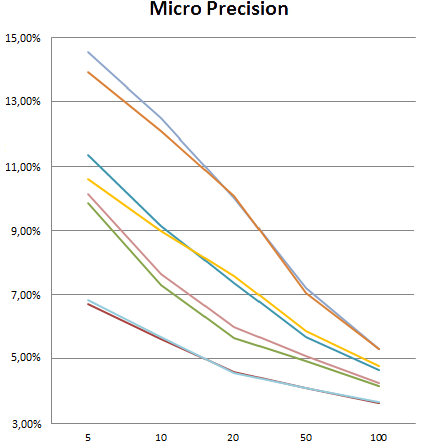
\includegraphics[width=.32\paperwidth]{./figure/graphs/Ottim_prec} 	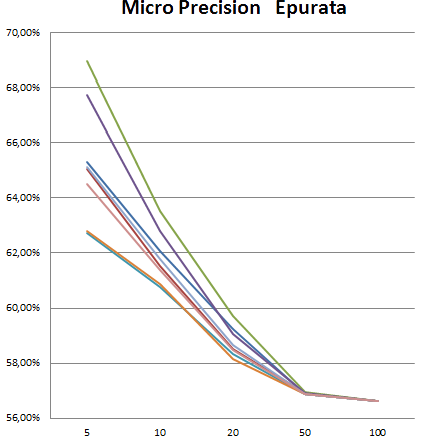
\includegraphics[width=.32\paperwidth]{./figure/graphs/Ottim_precT1}
%	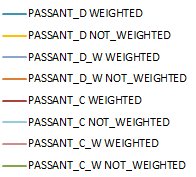
\includegraphics[width=.2\paperwidth]{./figure/graphs/legenda}
%\end{frame}

%%%%%%%%%%%%%%%%%%%%%%%%%%%%%%%%%%%%%%%%%%%%%%%%%%%%%

%\begin{frame}
%	\frametitle{Risultati - Configurazione 2}
%	\begin{tabular}{c c}	
%		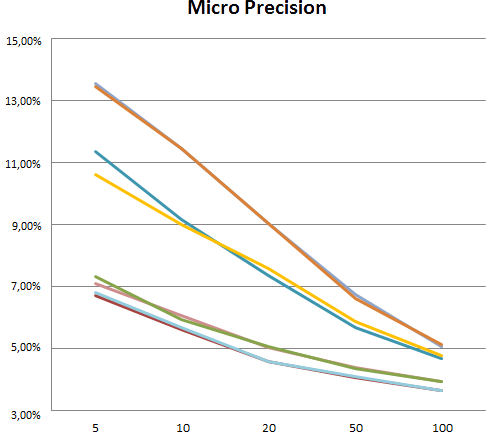
\includegraphics[width=.4\textwidth]{./figure/graphs/Nostra_prec} &
%		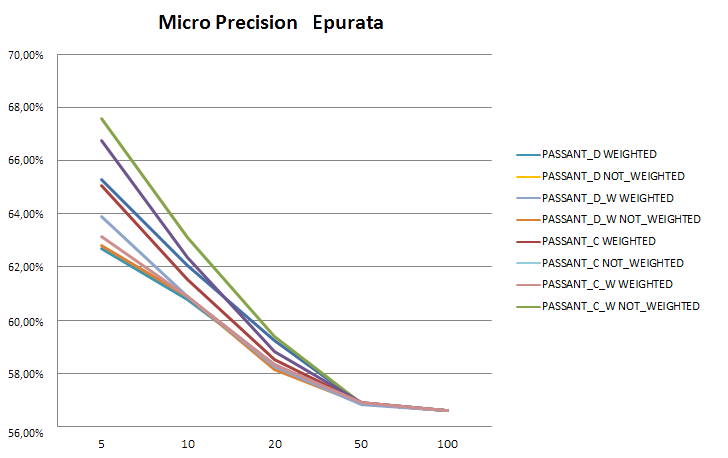
\includegraphics[width=.6\textwidth]{./figure/graphs/Nostra_precT} \\
%	\end{tabular}
%\end{frame}

%%%%%%%%%%%%%%%%%%%%%%%%%%%%%%%%%%%%%%%%%%%%%%%%%%%%%
%\begin{frame}
%	\frametitle{Risultati - Configurazione 3}
%	\begin{tabular}{c c}	
%		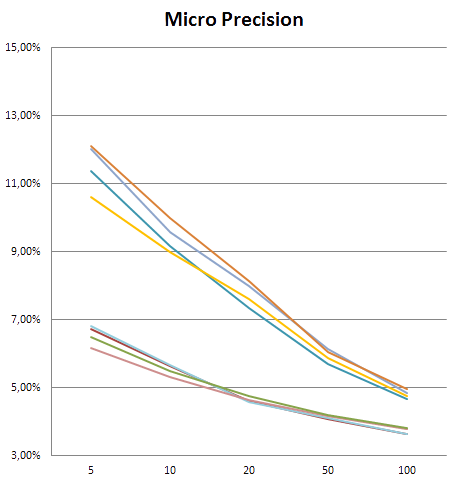
\includegraphics[width=.4\textwidth]{./figure/graphs/Musto_prec} &
%		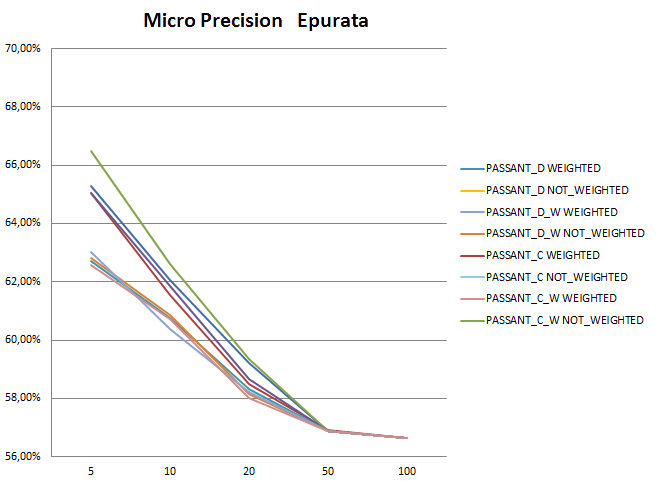
\includegraphics[width=.6\textwidth]{./figure/graphs/Musto_precT} \\
%	\end{tabular}
%\end{frame}

%%%%%%%%%%%%%%%%%%%%%%%%%%%%%%%%%%%%%%%%%%%%%%%%%%%%%
\begin{frame}
	\frametitle{$\mu$ Precision}
	\begin{columns}[htbp]
		\begin{column}{.68\paperwidth}
				\begin{tikzpicture}
				\begin{axis}[
				/tikz/font={\scriptsize},
				xmin=5,
				xmax=50,
			ymin=5,
			ymax=15,
			ylabel=$\mu\;precision (\%)$,
			xlabel= $k$,
			minor grid style={gray!30},
			major grid style={black!50},
			/pgfplots/xtick={5,10,20,50},
			/pgfplots/ytick={4,...,15},
			%yticklabel shift=0.5cm,
			%/pgfplots/ytick=data,
			grid=major,
			extra y ticks={4.1,4.2,...,4.9,5.1,5.2,...,5.9,
				6.1,6.2,...,6.9,7.1,7.2,...,7.9,8.1,8.2,...,8.9,
				9.1,9.2,...,9.9,10.1,10.2,...,10.9,11.1,11.2,...,11.9,
				12.1,12.2,...,12.9,13.1,13.2,...,13.9,14.1,14.2,...,14.9},
			mark=none,
			extra y tick style={yticklabels={},grid=minor,tiny,ytick pos=left},
				legend style={
					%font=\tiny,
					%pos=outer north east,
					%line width=.1pt,
					%mark size=.6pt
				},
				width=.9\textwidth,
				height=.8\textwidth,
				grid=both, 
				axis background/.style={fill=white}]
				\addplot[color=silver,thick] coordinates {
					(5,13.54)
					(10,11.44)
					(20,9.03)
					(50,6.73)
					%(100,5.06)
					
				};
				\addlegendentry{Config A} % conf A = nostra
				
				\addplot[color=bronze,thick] coordinates {
					(5,12.10)
					(10,9.98)
					(20,8.15)
					(50,6.04)
					%(100,4.85)
				};
				\addlegendentry{Config B} % conf B = musto
				
				\addplot[color=gold,thick] coordinates {
					(5,14.55)
					(10,12.51)
					(20,10.02)
					(50,7.20)
					%(100,5.31)
				};
				\addlegendentry{Config C} % conf C = max raggiunto
				
				\addplot[color=black,thick] coordinates {
					(5,11.35)
					(10,9.15)
					(20,7.35)
					(50,5.69)
					%(100,4.66)
				};
				\addlegendentry{\color{red}Baseline}
				\end{axis}
				\end{tikzpicture}				
		\end{column}
		\begin{column}{.3\paperwidth}
				\begin{itemize}
					\scriptsize
						\item +3.2 \% per $k = 5 $
						\item +3.36 \% per $k = 10 $
						\item +2.67 \% per $k = 20 $
						\item +1.51 \% per $k = 50 $
						%\item +0.65 \% per $k = 100 $			
				\end{itemize} 
		\end{column}
	\end{columns}
\end{frame} 
%%%%%%%%%%%%%%%%%%%%%%%%%%%%%%%%%%%%%%%%%%%
\begin{frame}
	\frametitle{$\mu$ Precision Epurata}
	\begin{columns}[htbp]
		\begin{column}{.68\paperwidth}
			\begin{figure}
				\begin{tikzpicture}
				\begin{axis}[
				/tikz/font={\scriptsize},
				xmin=5,
				xmax=50,
				ymin=56,
				ymax=69,
				ylabel=$\mu\;precision (\%)$,
				xlabel= $k$,
				minor grid style={gray!20},
				major grid style={black!40},
				/pgfplots/xtick={5,10,20,50},
				/pgfplots/ytick={56,...,69},
				%yticklabel shift=0.5cm,
				%/pgfplots/ytick=data,
				grid=major,
				extra y ticks={56.1,56.2,...,56.9,57.1,57.2,...,57.9,58.1,58.2,...,58.9,
					59.1,59.2,...,59.9,60.1,60.2,...,60.9,61.1,61.2,...,61.9,
					62.1,62.2,...,62.9,63.1,63.2,...,63.9,64.1,64.2,...,64.9,
					65.1,65.2,...,65.9,66.1,66.2,...,66.9,67.1,67.2,...,67.9},
				mark=none,
				extra y tick style={yticklabels={},grid=minor,tiny,ytick pos=left},
				legend style={
					%font=\tiny,
					%pos=outer north east,
					%line width=.1pt,
					%mark size=.6pt
				},
				width=.9\textwidth,
				height=.8\textwidth,
				grid=both, 
				axis background/.style={fill=white}]
				\addplot[color=silver,thick] coordinates {
					(5,67.57)
					(10,63.11)
					(20,59.37)
					(50,56.88)
					%(100,56.62)
					
				};
				\addlegendentry{Config A} % conf A = nostra
				
				\addplot[color=bronze,thick] coordinates {
					(5,66.49)
					(10,62.62)
					(20,59.36)
					(50,56.88)
					%(100,56.62)
				};
				\addlegendentry{Config B} % conf B = musto
				
				\addplot[color=gold,thick] coordinates {
					(5,68.97)
					(10,63.51)
					(20,59.72)
					(50,56.94)
					%(100,56.62)
				};
				\addlegendentry{Config C} % conf C = max raggiunto
				
				\addplot[color=black,thick] coordinates {
					(5,65.29)
					(10,62.06)
					(20,59.23)
					(50,56.88)
					%(100,56.62)
				};
				\addlegendentry{\color{red}Baseline}
				\end{axis}
				\end{tikzpicture}
			\end{figure}
		\end{column}
		\begin{column}{.3\paperwidth}
			\begin{itemize}
			\scriptsize
				\item +3.68 \% per $k = 5 $
				\item +1.45 \% per $k = 10 $
				\item +0.49 \% per $k = 20 $
				\item +0.06 \% per $k = 50 $
				%\item 0 \% per $k = 100 $			
			\end{itemize} 
		\end{column}
	\end{columns}
\end{frame}	
%%%%%%%%%%%%%%%%%%%%%%%%%%%%%%%%%%%%%%%%%%%
\section{Conclusioni e sviluppi futuri}
%%%%%%%%%%%%%%%%%%%%%%%%%%%%%%%%%%%%%%%%%%%

\begin{frame}
%	basicstyle=\fontsize{8}{10}\selectfont \ttfamily,%
\begin{center}
Grazie per l'attenzione.
\end{center}
\end{frame}
\end{document}
